% Created 2016-04-01 Fri 17:44
% Intended LaTeX compiler: pdflatex
\documentclass[11pt]{article}
\usepackage[utf8]{inputenc}
\usepackage[T1]{fontenc}
\usepackage{graphicx}
\usepackage{grffile}
\usepackage{longtable}
\usepackage{wrapfig}
\usepackage{rotating}
\usepackage[normalem]{ulem}
\usepackage{amsmath}
\usepackage{textcomp}
\usepackage{amssymb}
\usepackage{capt-of}
\usepackage{hyperref}
\usepackage{minted}
\usepackage[margin=0.75in]{geometry}
\newcommand{\norm}[1]{\Vert #1 \Vert}
\newcommand{\opnorm}[1]{\Vert #1 \Vert_{op}}
\newcommand{\fnorm}[1]{\Vert #1 \Vert_F}
\newcommand{\nucnorm}[1]{\Vert #1 \Vert_*}
\newcommand{\tr}{\operatorname{Tr}}
\newtheorem{theorem}{Theorem}[section]
\newtheorem{lemma}[theorem]{Lemma}
\newtheorem{proposition}[theorem]{Proposition}
\newtheorem{corollary}[theorem]{Corollary}
\newtheorem{proof}[theorem]{Proof}
\author{Bachir El khadir}
\date{\textit{<2016-03-11 Fri>}}
\title{Problem set 4, ORF523}
\hypersetup{
 pdfauthor={Bachir El khadir},
 pdftitle={Problem set 4, ORF523},
 pdfkeywords={},
 pdfsubject={},
 pdfcreator={Emacs 25.1.50.1 (Org mode )}, 
 pdflang={English}}
\begin{document}

\maketitle
\begin{HTML}

\label{orgspecialblock1}

\end{HTML}

\section{Problem 1}
\label{sec:orgheadline1}

Notations:
\begin{itemize}
\item \(c^*\) the solution to the problem. It exists because every subset of \(\mathbb R\) has a supremum.
\item \(X = (x_1, x_2, x_3, x_4)\)
\end{itemize}

\(f(X) =
X^T\begin{pmatrix}
 1          & -\frac12 & a           & \frac1{10}  \\
 -\frac12   & 1        & b           & c           \\
 a          & b        & 1           & -\frac3{10} \\
 \frac1{10} & c        & -\frac3{10} & 1           \\
\end{pmatrix}
X+\begin{pmatrix}2\\-a\\0\\c\end{pmatrix}^TX
:= X^TSX + w^TX\)


\begin{itemize}
\item If \(S\) is not nonnegative semi definite, there exist \(X\) such that \(X^TSX < 0\), and
\end{itemize}
$$f(\lambda X) = \lambda^2 X^TSX + \lambda w^TX \rightarrow_{\lambda \infty} -\infty$$
In order for the optimzation problem to be finite, we therefore need to have \(S \ge 0\).
\begin{itemize}
\item If \(S\) positive definite, Let \(\lambda_{\min}\) be its smallest eign value. Then
\(f(X) \ge \lambda_{\min}  ||X||^2 - ||w|| ||X|| \ge \lambda_{\min} (||X|| - \frac1{2\lambda_{\min}}||w||)^2 + cte\) is bounded from below.
\end{itemize}

Let \(c^+\) be the solution to the following convex optimization problem:
\(\max_{a, b, c, S \ge 0} c\)

\begin{minted}[frame=lines,linenos=true]{matlab}
n = 4
cvx_begin quiet
variable S(n,n) hermitian; 
variable a;
variable b;
variable c;

maximize(c);
S == hermitian_semidefinite( n );
for i = 1:4
    S(i, i) == 1 
end

S(1, 2) == -1/2;
S(1, 3) == a;
S(1, 4) == 1/10;
S(2, 3) == b;
S(2, 4) == c;
S(3, 4) == -3/10;
cvx_end

ans = [a b c]
\end{minted}

\begin{center}
\begin{tabular}{rrr}
-0.054543 & -0.22906 & 0.81168\\
\end{tabular}
\end{center}



\(0.8116 > c^+\)
For all \(c > c^+\), the optimization problem is not finite, so \(c^* \le c^+\).

Let \(c^- = 0.8115\), we check with CVX that
\[S =\begin{pmatrix}
 1          & -\frac12 & a^-           & \frac1{10}  \\
 -\frac12   & 1        & b^-           & c^-           \\
 a^-          & b^-        & 1           & -\frac3{10} \\
 \frac1{10} & c^-        & -\frac3{10} & 1           \\
\end{pmatrix}
 > 0
\]
with \(a^- = -0.0682\), \(b^- = -0.2216\)
The problem for \(c^-\) is then finite, so \(c^- <= c\).

Conclusion: 
$$0.9116 \le c^* \le 0.9117$$
or
$$c^* \approx 0.911$$

\section{Alternative way}
\label{sec:orgheadline2}

\[ S = \begin{pmatrix}
 1          & -\frac12 & a           & \frac1{10}  \\
 -\frac12   & 1        & b           & c           \\
 a          & b        & 1           & -\frac3{10} \\
 \frac1{10} & c        & -\frac3{10} & 1           \\
\end{pmatrix}\]

With a change of variable \(x_3 \leftrightarrow x_4\), we can rewrite \(S\):
\[Q = \begin{pmatrix}
 1          & -\frac12 &  \frac1{10}  & a\\
 -\frac12   & 1        &  c           & b\\
 \frac1{10} & c & 1 & -\frac3{10}\\
 a          & b        &  -\frac3{10} & 1
\end{pmatrix}\]

Note that \(Q \ge 0 \iff S \ge 0\), and \(Q > 0 \iff S > 0\).

In order of \(Q\) to be positive semi-definite, the following submatrix has to have a non-negative determinant:

\[  Q_1 = \begin{pmatrix}
 1          & -\frac12 &             \frac1{10}  \\
 -\frac12   & 1        &             c           \\
 \frac1{10} & c        &  1           \\
\end{pmatrix}\]

\begin{minted}[frame=lines,linenos=true]{matlab}
syms a b c;
S=[1,-1/2,a,1/10;-1/2,1,b,c;a,b,1,-3/10;1/10,c,-3/10,1];
Q_1 = [1 -1/2 1/10; -1/2 1 c; 1/10 c 1]
\end{minted}


\(det(Q_1) = g(c) = - c^2 - \frac1{10}c + \frac{37}{50}\)

It has two roots \(r_1 = \frac{-1 - 3\sqrt{33}}{10}, r_2 = \frac{-1 + 3\sqrt{33}}{10}\). Since the leadin coefficient is negative, the polynomial is non-negative iff \(c \in [r_1, r_2]\).

Let's now check that for \(c \in ]r_1, r_2[\), there exist \(a, b\) that make \(Q > 0\).
Indeed, by using Sylvester criterion:

\begin{itemize}
\item \(1 > 0\)
\item \[\det\begin{pmatrix}1&-\frac12\\-\frac12&1\end{pmatrix} = 1 - \frac14 > 0\]
\item \(det(Q_1) > 0\)
\end{itemize}

It remains to show that there exist to show that there exist \(a, b\) that make the following determinant positive:
\begin{align*}P(a, b) &:= \begin{vmatrix}
 1          & -\frac12 &  \frac1{10}  & a\\
 -\frac12   & 1        &  c           & b\\
 \frac1{10} & c & 1 & -\frac3{10}\\
 a          & b        &  -\frac3{10} & 1
\end{vmatrix}
\\&=
a^2c^2 - (3b)/100 - c/10 - ab - (3ac)/10 - (3bc)/5 - a^2 - (99b^2)/100 - c^2 - (3a)/50 - (abc)/5 + 269/400
\\&=
(c^2 - 1) a^2  -\frac{99}{100} b^2 - (\frac3{10}c + \frac3{50})a - (\frac3{100} + \frac35 c)b - (\frac{c}5+1) ab  - c^2 - c/10  + \frac{269}{400}
\\&=
-\begin{pmatrix}a\\b\end{pmatrix}^T
\underbrace{\begin{pmatrix}1-c^2&\frac{c}{10}+\frac12\\\frac{c}{10}+\frac12&\frac{99}{100}\end{pmatrix}\begin{pmatrix}a\\b\end{pmatrix}}_R
- \underbrace{\begin{pmatrix}\frac3{10}c + \frac3{50}\\ \frac3{100} + \frac35 c\end{pmatrix}}_{v}\begin{pmatrix}a\\b\end{pmatrix}
\underbrace{- c^2 - c/10  + \frac{269}{400}}_{\alpha}
\\&=
\begin{pmatrix}a\\b\end{pmatrix}^TR\begin{pmatrix}a\\b\end{pmatrix}
+v\begin{pmatrix}a\\b\end{pmatrix}
+ \alpha
\end{align*}

\(R\) is symmetric, By cholesky decomposition we can write it as \(R = U^TU\) 


\[U =\begin{pmatrix}
 \sqrt{1 - c^2}  &  \frac{c + 5}{10\sqrt{1 - c^2}}\\
               0 & \sqrt{\frac{g(c)}{1-c^2}}
\end{pmatrix}
\]


Let's do the change of variable \((x, y) = U(a, b)\):
\begin{align*}P(a, b)
&= -\begin{pmatrix}x\\y\end{pmatrix}^T\begin{pmatrix}x\\y\end{pmatrix} +(\underbrace{v^T{U^T}^{-1}}_{u^T})\begin{pmatrix}x\\y\end{pmatrix}+ \alpha
\\&= - (x+\frac{u_1}2)^2 - (y+\frac{u_2}2)^2 + \alpha + \frac{u_1^2}4 + \frac{u_2^2}4
\end{align*}

\begin{minted}[frame=lines,linenos=true]{matlab}
assume(c < 1/2 & c > 0)
R = [(1-c^2), (c/10 + 1/2); (c/10+1/2), 99/100];
U = chol(R, 'real');
u = v'*(U')^(-1);
\end{minted}

This polynomial can be non negative at some point if and only if \(\alpha + \frac{u_1^2}4 + \frac{u_2^2}4 \ge 0\), we use matlab to calculate that expression, we plot it:

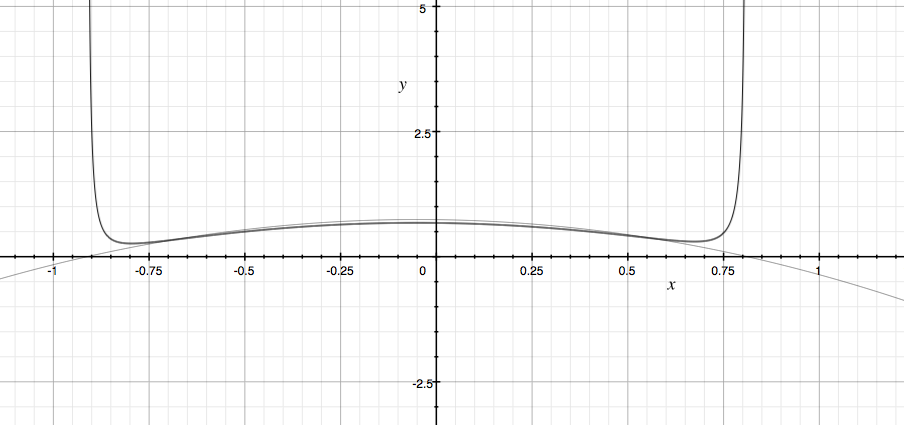
\includegraphics[width=.9\linewidth]{./poly.png}

Which shows that it is always positive between the roots.

\textbf{As a conclusion}:
\begin{itemize}
\item for \(r_1 < c < r_2\), there is \(a, b\) that make \(S > 0\), and therefore the problem bounded.
\item for \(c > r_2\), all \(a, b\) make \(S\) not semi-definite, and therefore the problem not bounded.
\item we conclude that \(c^* = r_2 = \frac{-1+3\sqrt{33}}{10}\)
\end{itemize}

\section{Problem 2}
\label{sec:orgheadline3}

\begin{enumerate}
\item Let  \(\Vert A\Vert _{\text{dual}} = \max_{\Vert X\Vert _{op} \le 1} \langle Y, X\rangle\) and let's prove that \(\Vert A\Vert _* = \Vert A\Vert _{\text{dual}}\)
\end{enumerate}
\begin{lemma}
If  \(A = U\Lambda V^T\) be the SVD decomposition of \(A\), then \(\nucnorm{A} = \tr(\Lambda)\)
\end{lemma}


\begin{itemize}
\item Let \(A = U\Lambda V^T\) be the SVD decomposition of \(A\), then \(\langle A, UV^T\rangle  = \tr(V \Lambda U^TUV^T) = \tr(V\Lambda V^T) = \tr(\Lambda) = \Vert A \Vert _*\). Note that \(\opnorm{UV^T} = 1\) because \(UV^T\) is orthogonal. We have just proved that  \(\Vert A\Vert _* \le \Vert A\Vert _{\text{dual}}\)
\end{itemize}


\begin{itemize}
\item Let \(X\) be a matrix st \(\opnorm{X} \le 1\), \(\langle A, X\rangle  = \tr(A^TX) = \tr(V \Lambda U^TX) = \tr(\Lambda U^TXV) = \sum \Lambda_{ii} (U^TXV)_{ii}  = \sum \Lambda_{ii} \underbrace{u_i^TXv_i}_{\le \Vert X\Vert _{op}} \le  \Vert X\Vert _{op} \Vert \Lambda\Vert _* \le \Vert A\Vert _*\). so  \(\Vert A\Vert _* \ge \Vert A\Vert _{\text{dual}}\)

\item As a conclusion \(\Vert A\Vert _* = \max_{\Vert X\Vert _{op} \le 1} \langle Y, X\rangle\), and \(\opnorm{.}\) is the dual of \(\nucnorm{.}\)
\end{itemize}


Let's now prove that the nuclear norm is indeed a norm:
\begin{itemize}
\item If \(\nucnorm{A} = 0\), then \(\forall i \le m \wedge n \; \sigma_i(A) = 0\), If \(U\Lambda V\) the SVD of A, then \(\Lambda = 0\), and therefore \(A = 0\).
\item If \(\alpha > 0\), \(\alpha A = U (\alpha \Lambda) V^T\), and therefore \(\nucnorm{\alpha A} = \tr(\alpha \Lambda) = \alpha \tr(\Lambda) = \alpha \nucnorm{A}\)
\item If \(\alpha < 0\), \(\alpha A  = (-U) (-\alpha \Lambda) V^T\), we conclude in the same way as before.
\item \(\nucnorm{A + B} = \max_{\opnorm{X} \le 1} <A + B, X> = \max_{\opnorm{X} \le 1} <A, X> + <B, X> \le  \max_{\opnorm{X} \le 1} <A, X> +  \max_{\opnorm{X} \le 1} <B, X>\) (Where we have used the fact that \(\sup(S_1+S_2) \le \sup S_1 + \sup S_2\) for any two sets \(S_1, S_2\)), so \(\nucnorm{A+B} \le \nucnorm{A} + \nucnorm{B}\)
\end{itemize}


\begin{enumerate}
\item 
\end{enumerate}

Let's first find unit sphere

\(A = \begin{pmatrix}x&y\\y&z\end{pmatrix}\), Let \(\lambda_1, \lambda_2\) be its eigen values.

\begin{align*}
\nucnorm{A} = 1
& \iff |\lambda_1| + |\lambda_2| = 1
\\ &\iff \lambda_1^2 + \lambda_2^2 + 2|\lambda_1\lambda_2| = 1
\\ &\iff (\lambda_1 + \lambda_2)^2 + - 2\lambda_1 \lambda_2 + 2 |\lambda_1\lambda_2| = 1
\\ &\iff \tr(A)^2  + 2 (|det(A)| -det(A)) = 1
\\ &\iff (\tr(A)^2  = 1 \text{ and } \det(A) \ge 0) \text{ or }  (\tr(A)^2 - 4 det(A) = 1 \text{ and } \det(A) \le 0)
\\ &\iff ((x+z)^2  = 1 \text{ and } xz \ge y^2) \text{ or }  ((x+z)^2 - 4 (xz-y^2) = 1 \text{ and } xz \le y^2)
\\ &\iff ((x+z)^2  = 1 \text{ and } xz \ge y^2) \text{ or }  ((x-z)^2 + 4 y^2 = 1 \text{ and } xz \le y^2)
\end{align*}


Let's do the linear change of variable

\begin{align*}
u &= \frac{x + z}{\sqrt 2}\\
v &= \sqrt2 y\\
w &= \frac{x - z}{\sqrt 2}\\
\end{align*}

Which can also be written in matrix form as:

\[\begin{pmatrix}u\\w\\v\end{pmatrix}=\underbrace{\begin{pmatrix}
cos(-\frac{\pi}4)&-sin(-\frac{\pi}4)&0\\
sin(-\frac{\pi}4)&cos(-\frac{\pi}4)&0\\
0&0&\frac1{\sqrt2}\\
\end{pmatrix}}_{R}
\begin{pmatrix}x\\z\\y\end{pmatrix}\]
The linear transformation \(R\) is then a rotation of \(-\frac{\pi}4\) in the \((X, Z)\) plane, and a scaling of \(\frac1{\sqrt2}\) along the \(Y\) axis.

To find the shape of the unit cylinder, we work in the \((u, v, w)\) space, and then we apply to inverse transformation of \(R\).


Then \(2xz = u^2 - w^2\), and
\begin{align*}
\nucnorm{A} = 1
&\iff (2 u^2 = 1 \text{ and } u^2 - w^2 \ge v^2) \text{ or }  (2 w^2 + 2 v^2 = 1 \text{ and } u^2 - w^2 \le v^2)
\\&\iff (u^2 = \frac12 \text{ and } u^2 \ge v^2 + w^2) \text{ or }  (w^2 + v^2 = \frac12 \text{ and } u^2 \le v^2 + w^2)
\\&\iff (u = \pm \frac12 \text{ and } \frac12 \ge v^2 + w^2) \text{ or }  (w^2 + v^2 = \frac12 \text{ and }-\frac12 \le u \le \frac12)
\end{align*}

\(\{u = \pm \frac12 \text{ and } \frac12 \ge v^2 + w^2\}\) is two centered disks of radius \(\frac1{\sqrt2}\) in the plane \(u=\pm \frac12\) .
\(\{w^2 + v^2 = \frac12 \text{ and }-\frac12 \le u \le \frac12\}\) is the lateral surface of the cylinder of radius \(\frac1{\sqrt 2}\) and axis \(u\)

\textbf{Conclusion:} In \((u, v, w)\) space, the unit sphere \(S(0, 1)\) is the basis and lateral surface of the cylinder with radius \(u\), radius \(\frac1{\sqrt2}\), and height \(1\).


\begin{lemma}
The unit ball \(B(0, 1)\) is the convex hull of the unit sphere \(S(0, 1)\).
\end{lemma}
\(B(0, 1)\) is convex containing \(S(0, 1)\). If \(x, y \in S(0, 1)\), and \(\alpha \in (0, 1)\), then \(|\alpha x + (1-\alpha)y|_* \le \alpha |x|_* + (1-\alpha) |y|_* \le 1\) because of the triangular inequality. 

\(B(0, 1)\) is then a cylinder.


\begin{minted}[frame=lines,linenos=true]{python}
import matplotlib
import matplotlib.pyplot as plt
from mpl_toolkits.mplot3d import Axes3D
import np

num_points = 30

# Construct cylinder
# base
x=np.linspace(-1,1,num_points)
z=np.linspace(-1,1,num_points)
X, Z=np.meshgrid(x,z)
Y=np.sqrt(1-X**2)

P = map(lambda u: u.ravel(), [X, Y, Z])
P[0] = np.concatenate((P[0], X.ravel()))
P[1] = np.concatenate((P[1], (-Y.ravel())))
P[2] = np.concatenate((P[2], Z.ravel()))

# lateral surface
t=np.linspace(0,1,num_points)
theta=np.linspace(0, 2*np.pi,num_points)
T, Theta = np.meshgrid(t, theta)

X = np.cos(Theta)*T
Y = np.sin(Theta)*T
Z = X*0 + 1
P[0] = np.concatenate((P[0], X.ravel()))
P[1] = np.concatenate((P[1], Y.ravel()))
P[2] = np.concatenate((P[2], Z.ravel()))

P[0] = np.concatenate((P[0], X.ravel()))
P[1] = np.concatenate((P[1], Y.ravel()))
P[2] = np.concatenate((P[2], -Z.ravel()))

# Inverse tranformation
R = np.array([[1, 0, 1], [0, 2, 0], [1,0,-1]]) / np.sqrt(2)
P = np.array(P)
P = np.dot(np.linalg.inv(R), P)

# Plot
fig = plt.figure()
ax = fig.add_subplot(111, projection='3d')
ax.scatter(*P)
plt.xlabel('x')
plt.ylabel('y')
plt.zlabel('z')
plt.show()
fig.savefig('cylinder.png')
\end{minted}

\begin{center}
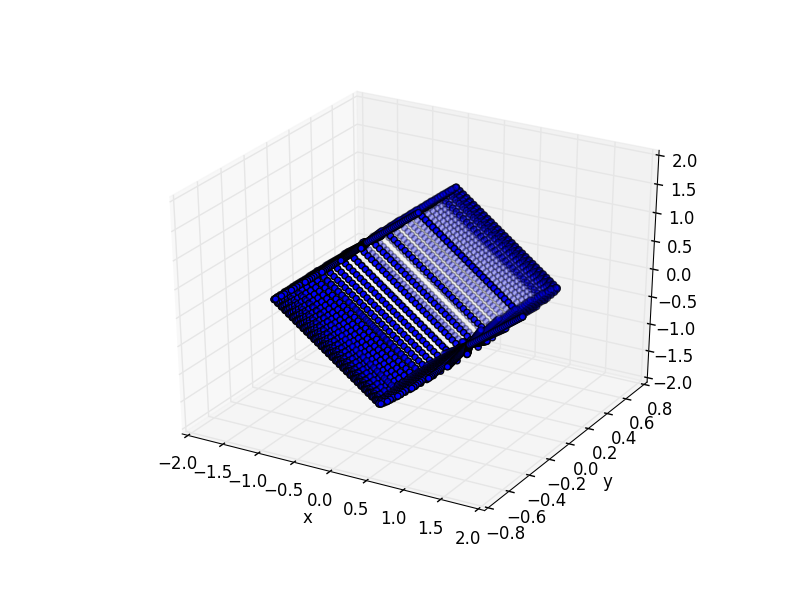
\includegraphics[width=0.5\textwidth]{./cylinder.png}
\captionof{figure}{Shape of the unit nuclear ball}
\end{center}


\textbf{3.}
\begin{lemma}
For \(Y \in \mathbb R^{n\times m}\)
$$||Y||_{op} \le 1 \iff \begin{pmatrix}I_n&Y\\Y^T&I_m\end{pmatrix} \ge 0$$
\end{lemma}
Proof: \(||Y||_{op} \le 1 \iff \forall x \in \mathbb{R^m} \le 1 x^TY^TYx \le x^TI_mx \iff Y^TI_nY \le I_m\) We conclude by Schur lemma.


Back to the problem, we can write the nuclear norm as a solution to an SDP:
\begin{align*}
.||X||_* = \max_{||Y||_{op} \le 1} <X, Y>
&= \max_{\begin{pmatrix}I_n&Y\\Y^T&I_m\end{pmatrix} \ge 0} <X, Y>
\\&= \max_{\underbrace{\begin{pmatrix}I_n&Y\\Y^T&I_m\end{pmatrix}}_Z \ge 0} <X, Y>
\\&= \frac12 \max_{Z \ge 0, Z \in C}  < \underbrace{\begin{pmatrix}0&X\\X^T&0\end{pmatrix}}_{X'}, Z>
\end{align*}

Where
\begin{itemize}
\item \(C = \{Z \in \mathbb R^{(n+m)\times(n+m)} : <E_{ij},Z> = 1_{i = j} \text{ for } (i, j) \in \mathcal I \}\) is a set defined by affine inequalities
\item \(E_{ij}\) is the \((n+m)\times(n+m)\) matrix with 0 every where except on the entries \((i,j)\) and \((j, i)\) where it is equal to 1.
\item \(\mathcal I = \{ (i, j) \in [1, n+m]^2, ((i \vee j) \le n) \text{ or } (n < (i \wedge j))\}\)
\end{itemize}

The feasible set \(\{Z \ge 0, Z \in C\} \equiv \{Y : ||Y||_{op} \le 1\}\) is the unit ball of a norm, so it is strictly feasible.

The dual of this SDP can then be written as:

\(\min_{\mu \in \mathbb R^{\mathcal I}, \sum_{(i,j) \in I} \mu_{ij} E_{ij} \ge X'} <\mu, b>\)

Where \(b_{ij} = 1_{ij}\)

The feasible set of this program can be written as:

$$\{ (\mu_1, \mu_2) \in \mathbb R^{n\times n} \times \mathbb R^{m \times m} \begin{pmatrix}\mu_1&X\\X^T&\mu_2\end{pmatrix} \ge 0\}$$

This set also strictly feasible, indeed, since adding \(t\) times the identity matrix shift all the eigen values, for \(t \in \mathbb R\) large enough, we have that:

\(\begin{pmatrix}tI_n&X\\X^T&tI_m\end{pmatrix} > 0\)


This proves that the primal and dual are equal.

Now, we can rewrite the originial problem \(\min_{\mathcal A(X) = c} |X|_*\) where \(\mathcal A\) any linear functional as:
\(\min_{\mathcal A(X) = c} |X|_* = \min_{\mathcal A(X) = c} \max_{|Y|_{op} \le 1} <X, Y> =  \min_{X, \mu, \mathcal A(X) = c, \sum \mu_i A_i \ge X'} \mu^T b\)
Where \(b, X'\) are the same as defined above. This is obviously an SDP.

\section{Problem 3}
\label{sec:orgheadline4}

\textbf{1.}

Let's first show the following:
\begin{lemma}
a Matrix \(D\) is a distance matrix of somes points \(x_1, \ldots, x_n\) iff there exist \(X \ge 0, X \in \mathbb R^{m \times m}\) such that \(D_{ij} = X_{ii} + X_{jj} - 2X_{ij}\) 
\end{lemma}
Indeed, if \(D\) is the distance matrix of \(x_1, \ldots, x_n\), let \(X = (<x_i, x_j>)_{ij}\). Then:
\begin{itemize}
\item \(D_{ij} = ||x_i - x_j||^2 = <x_i, x_i> + <x_j, x_j> - 2 <x_i, x_j> = X_{ii} + X_{jj} - 2 X_{ij}\).
\item \(X\) is symmetric because \(<.,.>\) is symmetric.
\item Let \(y \in \mathbb R^n\)  \(y^TXy = \sum_{ij} <x_i, x_j> y_iy_j = ||\sum y_i x_i||_2^2 \ge 0\), so \(X \ge 0\)

For the converse, let \(X\) a psd such that \(D_{ij} = X_ii + X_jj - 2X_{ij}\). By Cholesky decomposition, let \(M = \begin{pmatrix}m_1^T\\\vdots\\m_n^T\end{pmatrix} \in \mathbb R^{n \times n}\) s.t \(X = MM^T\), eg \(X_{ij} =m_i^Tm_j\), so that \(D_{ij} = ||m_i - m_j||^2\)

Using this Lemma, to solve the problem we have the check only if \(D\) can be written as  \(D_{ij} = X_{ii} + X_{jj} - 2X_{ij}\) for some matrix \(X \ge 0\).
e.g. check if the following SDP is feasible $$\{X \ge 0; D_{ij} = X_{ii} + X_{jj} - 2X_{ij}\}$$.
\end{itemize}


\textbf{2.}
Take
$$D = \begin{pmatrix}
   0 & 1 & 1 & 1\\
   1 & 0 & 1 & 1\\
   1 & 1 & 0 & 2\\
   1 & 1 & 2 & 0\\
  \end{pmatrix}
  $$
It trivially verifies the triangular inequality.

Suppose it is a distance matrix, then by the lemma, there exist 4 points \(x_1, x_2, x_3, x_4\) in \(\mathbb R^4\)
such that \(||x_i - x_j|| = D_{ij}, i,j=1,\ldots,4\)

\begin{itemize}
\item \(x_2, x_3, x_4 \in B(x_1, 1)\)
\item \(|x_4-x_3| = 2\), so \([x_4, x_3]\) is a diameter in \(B(x_1, 1)\), so \(x_1 \in \frac{x_3 + x_4}2\)
\item \(|x_2 - x_4| + |x_2 - x_3| = 1 + 1 = |x_4 - x_3|\), so \(x_2 \in [x_3, x_4]\), so \(x_2 = \frac{x_4 - x_3}2 = x_1\)
\item But \(|x_2 - x_1| = 1 \ne 0\), contradiction

Concolusion: \(D\) is not a distance matrix.
\end{itemize}

\section{Problem 4}
\label{sec:orgheadline5}


\textbf{1.}

\(A_1 = \begin{pmatrix} 0 & 1 \\ 0 & 0 \end{pmatrix}\)

\(A_2 = \begin{pmatrix} 0 & 0 \\ 1 & 0 \end{pmatrix}\)

\(A_2 A_1 = \begin{pmatrix}0& 0\\0&1\end{pmatrix}\)


\(A_1, A_2\) and \(A_2A_1\) are triangular, so the eigen values are all in the diagonal,  e.g \(\rho(A_1) = \rho(A_2) = 0\), but , \(\rho(A_2A_1) = 1\).

\textbf{2.}

The following program:
\begin{minted}[frame=lines,linenos=true]{matlab}
A1 = [-1 -1; -4 0] / 4;
A2 = [3 3; -2 1] / 4;

cvx_begin sdp
variable P(2, 2)
minimize(P(2, 1))
P >= 1
A1 * P * A1' <= P
A2 * P * A2' <= P
cvx_end

ans=P
\end{minted}

proves that there exist \(P \ge 0\)  such that:

\(A_1' P A_1 \le P, A_2' P A_2 \le P\)


\begin{lemma}
Let \(A, B \ge 0\), If \(A \ge 0\), then \(B'AB \ge 0\)
\end{lemma}


\begin{proof}
Indeed, for \(x \in \mathbb R^n\), \(x'B'ABx = (Bx)' A (Bx) \ge 0\)
\end{proof}

Let \(\Sigma\) be a product of term of the form \(A_1\) or \(A_2\)

Let's prove by induction on the size on the number of terms \(\Sigma\), that \(\Sigma' P \Sigma \le P\).

Indeed, let \(\Sigma\) be of size \(n+1\), without loss of generality \(\Sigma = \Sigma_1 A_1\), with \(\Sigma_1\) of size \(n\).

Then \(\Sigma' P \Sigma = A_1' \underbrace{\Sigma_1' P \Sigma_1}_{\le P} A_1 \le A_1' P A_1 \le A_1\).

By lyapounouv theorem, \(\Sigma\) is then stable, or equivalenty \(\{A_1, A_2\}\) is stable.
\end{document}